\documentclass[12pt, oneside]{article}
\usepackage[letterpaper, margin=1in, headsep=0.5in]{geometry}
\usepackage[english]{babel}
\usepackage[utf8]{inputenc}
\usepackage{amsmath}
\usepackage{amsfonts}
\usepackage{amssymb}
\usepackage{tikz}
\usetikzlibrary{angles}
%\usepackage{pgfplots}
%\pgfplotsset{width=10cm,compat=1.9}



%\usepackage{tkz-fct} %alternative to pgfplots.
%\usepackage{pgfplots}
%\pgfplotsset{width=10cm,compat=1.9}
%\usepgfplotslibrary{statistics}
%\usepackage{pgfplotstable}
%\usepackage{venndiagram}


\begin{document}
\begin{enumerate}

\item Draw and label the geometric object $\overrightarrow{AB}$
\vspace{2cm}


\item Given line $\overleftrightarrow{AB}$ with midpoint $M$, that is, $\overline{AM} \cong \overline{BM}$. $AM=2$ cm. Find the length of $\overline{AB}$.\\[0.75cm]
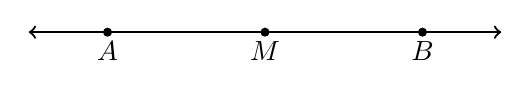
\begin{tikzpicture}
  \centering
  \draw [<->, thick] (0,0)--(6,0); % also thin, ultra thick, help lines, dashed, dotted, red
  \draw [fill] (1,0) circle [radius=0.05] node[below]{$A$};
  \draw [fill] (5,0) circle [radius=0.05] node[below]{$B$};
  \draw [fill] (3,0) circle [radius=0.05] node[below]{$M$};
\end{tikzpicture}
\vspace{3cm}

\item Given $\triangle ABC$ with $\overline{AC} \cong \overline{BC}$. On the diagram mark the congruent line segments with tick marks.\\[0.5cm]
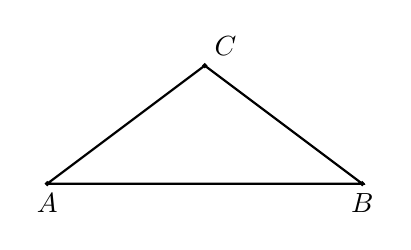
\begin{tikzpicture}[scale=0.5]
  \draw [thick](0,0)--(8,0)--(4,3)--(0,0);
  \draw [fill] (0,0) circle [radius=0.05] node[below]{$A$};
  \draw [fill] (8,0) circle [radius=0.05] node[below]{$B$};
  \draw [fill] (4,3) circle [radius=0.05] node[above right]{$C$};
\end{tikzpicture}

\item Given $\triangle ABC$ with $\overline{AC} \cong \overline{BC}$. $AC=x+7$ and $BC=2x+1$. Find $AC$.\\[0.5cm]
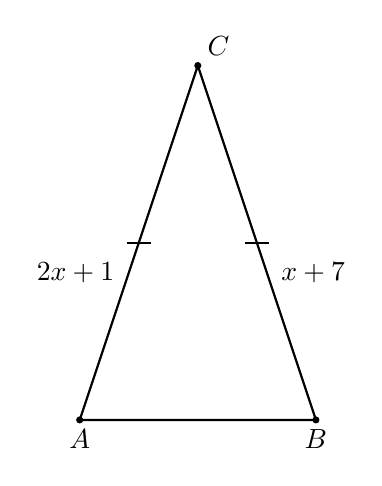
\begin{tikzpicture}[scale=0.75]
  \draw [thick](0,0)--(4,0)--(2,6)--(0,0);
  \draw [fill] (0,0) circle [radius=0.05] node[below]{$A$};
  \draw [fill] (4,0) circle [radius=0.05] node[below]{$B$};
  \draw [fill] (2,6) circle [radius=0.05] node[above right]{$C$};
  \draw [thick] (0.8,3)--(1.2,3); %tick mark
  \draw [thick] (2.8,3)--(3.2,3); %tick mark
  \node [right] at (3.25,2.5){$x+7$};
  \node [left] at (0.75,2.5){$2x+1$};
\end{tikzpicture}

\item Given $\overrightarrow{DE}$, construct circle $E$ with radius $DE$.
\vspace{4cm}
\begin{center}
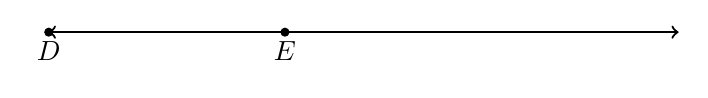
\begin{tikzpicture}
  \draw [<->, thick] (0,0)--(8,0);
  \draw [fill] (0,0) circle [radius=0.05] node[below]{$D$};
  \draw [fill] (3,0) circle [radius=0.05] node[below]{$E$};
\end{tikzpicture}
\end{center}

\item big skip
\bigskip

\item small skip follows
\smallskip
\item the end

\end{enumerate}
\end{document}
